\documentclass[../thesis.tex]{subfiles}

\begin{document}

\begin{figure}
  \centering
  \begin{subfigure}[b]{0.3\linewidth}
    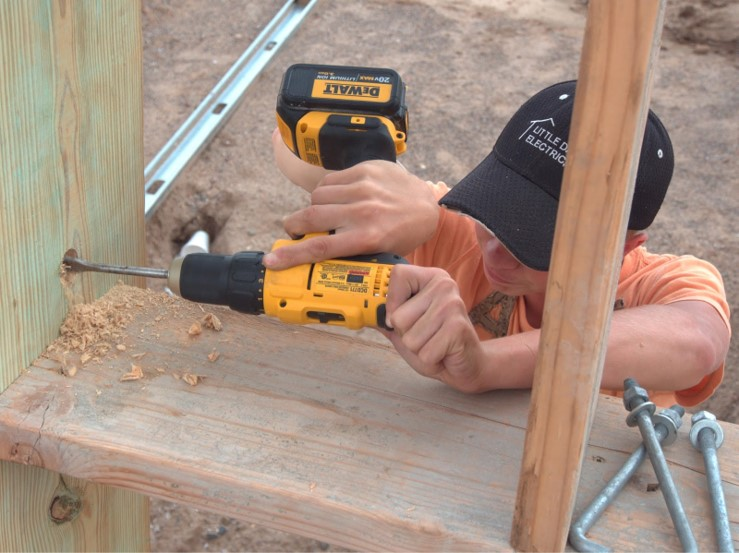
\includegraphics[width=\linewidth]{./Introduction/Drill.jpg}
  \end{subfigure}
  \hfill
  \begin{subfigure}[b]{0.3\linewidth}
    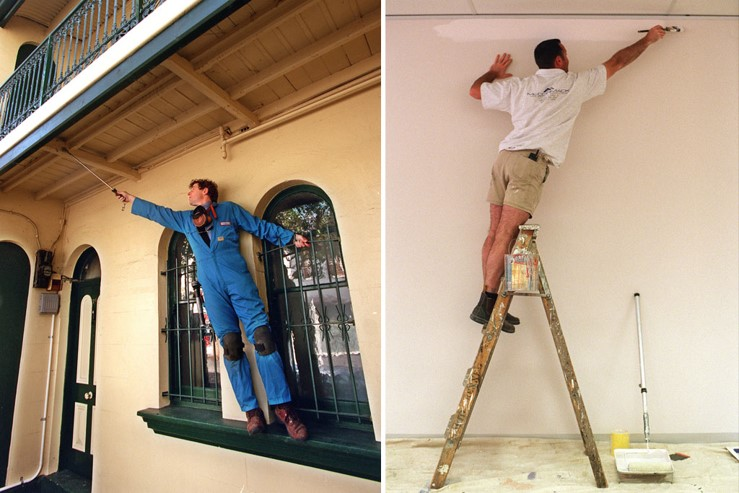
\includegraphics[width=\linewidth]{./Introduction/ladder.jpg}    
  \end{subfigure}
  \hfill
  \begin{subfigure}[b]{0.3\linewidth}
    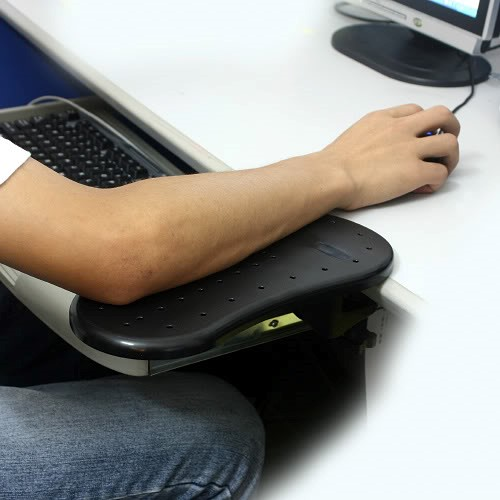
\includegraphics[width=\linewidth]{./Introduction/mouse.jpg}    
  \end{subfigure}
  \label{fig:HumanContact}
  \caption{Humans using contact to improve reach, accuracy, and stability}    
\end{figure}



Contacting the world can provide stability, support, and sensory information.
Humans benefit from touching the world in situations from blindly detecting an object in the back of the refrigerator, to leaning on a stair railing. 
In the recent DARPA robotics challenge top robotics research teams from around the world submitted robots to attempt an obstacle course of challenges.
Many of these robots fell on the stairs. 
Not a single robot used the railing \cite{Atkeson2015}.
Even drunk people know to use railings, so there is plenty of room for improvement in robotics.

However, in robotics there are good reasons to avoid contact with the environment.
Hitting the world can provide large forces that destabilize or break the robot.
Relying on contacts can be dangerous as slight alterations in the world or errors in robot position may drastically alter the contact forces.
Instead of firmly grasping a handle, a few centimeters of error have caused robots to embarrassingly grasp air and fall over \cite{DarpaRoboticsVideo}.
Even when working entirely in simulation contacts between rigid bodies cause problems for physics engines.


Contacts introduce non-smooth discontinuities, which presents a challenge for many tools in the roboticists arsenal.
The benefits of contacts occur on a measure-zero manifold in the robot's configuration space.
For example, hand rests comfortably on a table at a specific configuration of shoulder, elbow, and wrist positions.
A slight extension of the elbow while fixing all other joints leads to the hand puncturing the table, while a slight contractions pulls the hand into the air and the table might as well not exist.
Random sampling and gradient decent are two techniques that appear in the solution to many robotics challenges, but both have difficulty with these measure-zero contact manifolds.
This thesis explores and extends techniques of sampling based and gradient methods to the problems of localization and planning, with the addition of contact forces and measurements.


%% Standard numerical techniques of discretization fail to capture the near instantaneous effects of contact both in modeling uncertainty and planning.


\section{Motivation}
My personal motivation for the topics covered in this thesis come, in part, from my past experience as a robotics engineering building robots that build airplanes.
Currently, large robotic arms equipped with expensive, specialized end effectors perform a variety of tasks for aerospace manufacturing, including drilling holes, inserting fasteners, milling, carbon fiber placement and layup, and sealant application.
While there are many potential directions of research to improve these already impressive machines, two striking issues are addressed by my work.

\subsection{Jigs are More Expensive Than Robots}

\begin{figure}
  \centering
  \begin{subfigure}[b]{0.586\linewidth}
    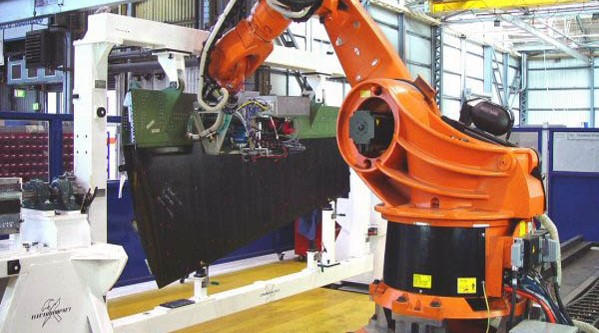
\includegraphics[width=\linewidth]{./Introduction/Robot1Outside.jpg}    
  \end{subfigure}
  \hfill
  \begin{subfigure}[b]{0.4\linewidth}
    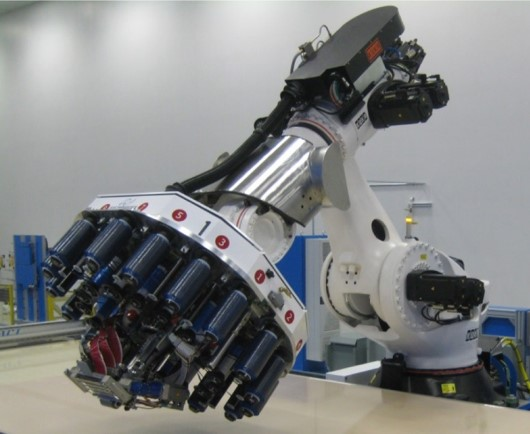
\includegraphics[width=\linewidth]{./Introduction/Robot2Outside.jpg}    
  \end{subfigure}
  \label{fig:KukaRobots}
  \caption{Robots working on the outside of parts held firmly in jigs}
\end{figure}

Robots that perform one type of task on one section of an airplane can cost millions of dollars.
However the jig that holds the airplane section while the robot works can cost more than the robot.
These jigs may have more actuators and tighter tolarances than the robotic system.
When the robot begins work on a new section, before ever making a measurement the jig has already located the part to within a few inches.
A few scripted measurement with a probe, programmed by an engineer, are sufficient to fully localize the part to within the needed tolerances.
%% These high costs and skilled engineering time are only acceptable because the expense is amortized over many
When amortized over many airplanes the per-part cost drops.
However, this process is inflexible and poorly suited to low-rate manufacturing.

If the robot could localize the part from a wide range of part configurations, and if the robot could reason about interal assembly tolerances then jigs could be make more cheaply, robots would become more versitile, less part-specific programming would be required, and machining accuracy could improve.

\subsection{Robots Stay on the Outside}

\begin{figure}
  \centering
  \label{fig:PeopleInWing}
  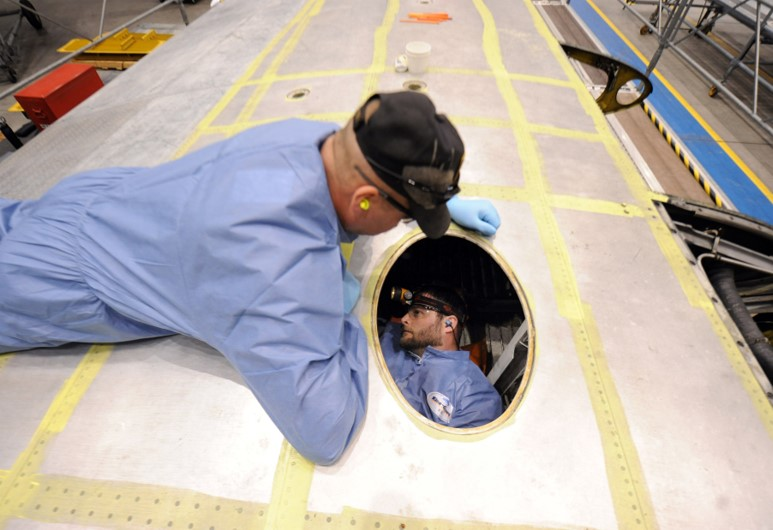
\includegraphics[width=.7\linewidth]{./Introduction/PeopleInWing.jpg}  
  \caption{Workers crawling in the confined spaces of an airplane wing}
\end{figure}

Large robotic arms cannot fit in the convined spaces of an aircraft.
While a team of people may include workers on both the inside and outside, large robots are limited to just the outside.



\section{Contribution}

\section{Thesis Outline}



\end{document}
